Where normal thresholding uses only one value for an entire image, adaptive threshold allows for the thresholding value to change according to the surroundings. This is very good for operations that take place in scenes with different light and thereby it is more robust.

Normal thresholding is a very simple operation.\\

\begin{center}
	if $P(x,y) > threshold$ then $P(x,y) = 1$

	else $P(x,y) = 0$\\
\end{center}

Using adaptive threshold it becomes slightly more complicated. The threshold is now no longer static, but dynamic and depends on the surrounding pixels in a blocksize $b$. The blocksize $b$ is a value that determine how big a portion of the surroundings the threshold will be calculated from.\\

\begin{center}
	$threshold = \sum_{k=x-b}^{x+b} \sum_{j=y-b}^{y+b} P(x,y)$

	$if  P(x,y) > threshold$ then $P(x,y) = 1$

	else $P(x,y) = 0$
\end{center}


Furthermore it is possible to select if the mean should be a equally weighted mean or if it should be a gaussian mean which would put the closest pixels to more importance.

An example of using adaptive threshold can be seen here and it is easy to see the big advantage of adaptive threshold\ref{fig:adaptivethreshold}. 

\begin{figure}[htpb]
\begin{center}
\leavevmode
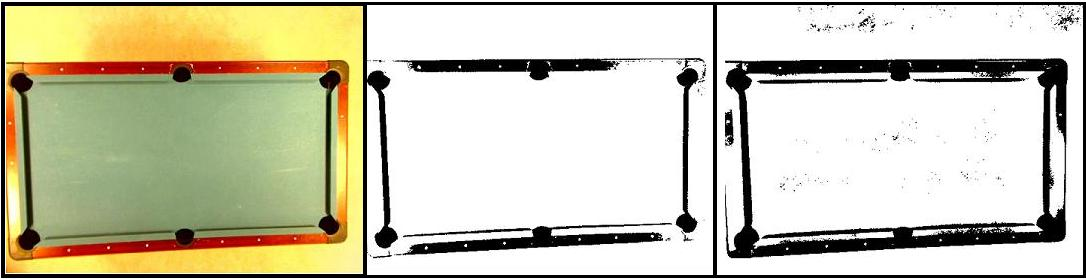
\includegraphics[width=1\textwidth]{images/adaptive_threshold.JPG}
\end{center}
\caption{First image not processed, second is normal threshold and third is using adaptive threshold}
\label{fig:adaptivethreshold}
\end{figure}

In this example the objective was to find the diamonds and the is better accomplished using adaptive threshold. If the light would have been the same in every part of the input image then normal threshold would have been just as good, but the light often would not be. The noise introduced by adaptive thresholding, as seen in the top right corner, can easily be removed with a standard median filter.